%Se abre la veda. Sin piedad con él paper!

\documentclass{llncs}
\usepackage{graphics}
\usepackage[dvips]{epsfig}
\usepackage[latin1]{inputenc}
\usepackage{color}
\usepackage{longtable}
%\usepackage{multirow}
\usepackage[dvips]{graphicx} 
%\usepackage{amsmath}
\usepackage{textcomp}
\usepackage{url}
\usepackage{algpseudocode}
\usepackage{caption}
\usepackage{subcaption}

\captionsetup{compatibility=false}

\newcommand{\tab}{\hspace{20mm}}

\setlength{\textfloatsep}{8pt plus 2pt minus 2pt}
\setlength{\intextsep}{8pt plus 2pt minus 2pt}

%#\def\BibTeX{{\rm B\kern-.05em{\sc i\kern-.025em b}\kern-.08em
%#    T\kern-.1667em\lower.7ex\hbox{E}\kern-.125emX}}

%\hyphenation{}

\begin{document}

%%%%%%%%%%%%%%%%%%%%%%%%%%%%%%%   TITLE   %%%%%%%%%%%%%%%%%%%%%%%%%%%%%%%

\title{Co-Evolutionary Optimization of Autonomous Agents in a Real-Time Strategy Game}
% autonomous por qué? Por qué no simplemente playing?

%OK, no revisamo0s, pero para eso mejor haz una rama y trabaja con la
%rama. No cambies nombres que despista. - JJ

\titlerunning{Co-Evolutionary Optimization of Bots in an RTS}


%%%%%%%%%%%%%%%%%%%%%%%%%%%%%%%   AUTHORS   %%%%%%%%%%%%%%%%%%%%%%%%%%%%%%%

%\author{A. Fernández-Ares \and A.M. Mora \and  J.J. Merelo \and \\ P. García-Sánchez \and P.A. Castillo}
%\authorrunning{A. Fernández-Ares. et al.}
%
%\institute{Departamento de Arquitectura y Tecnolog\'{\i}a de Computadores.\\
%Universidad de Granada (Spain)\\
%\email{antares.es@gmail.com}, \\ \email{\{amorag,jmerelo,pgarcia,pedro\}@geneura.ugr.es}
%}

\maketitle

%
%%%%%%%%%%%%%%%%%%%%%%%%%%%%%%%   ABSTRACT   %%%%%%%%%%%%%%%%%%%%%%%%%%%%%%%
%
\begin{abstract}
This paper presents an approach based in an evolutionary algorithm, aimed to improve the behavioral parameters which guide the
actions of an autonomous agent (bot) inside the real-time strategy game, Planet Wars. 

The work describes a co-evolutionary implementation of a
previously presented method (GeneBot), which yielded successful results, but focused in 4 vs 4 matches this time.
% Maribel, quita GeneBot y pon FooBot para el doble ciego

Thus, there have been analyzed the effects of considering several individuals
to be evolved (improved) at the same time in the algorithm, along with the use of three different fitness functions measuring the goodness of each bot in the evaluation. They are based in turns and position, and also in mathematical computations of linear regression and area regarding the number of ships belonging to the bot/individual to be evaluated.

In addition, the variance of using an evolutionary algorithm with and without previous knowledge in the co-evolution phase is also studied, i.e., respectively using specific rivals to perform the evaluation, or just considering to this end individuals in the population being evolved.

The aims of these co-evolutionary approaches are mainly two: first, reduce the computational time; and second find a robust fitness function to be used in the generation of evolutionary bots optimized for 4 vs 4 battles.

\end{abstract}

%
%%%%%%%%%%%%%%%%%%%%%%%%%%%%%%%   INTRODUCTION   %%%%%%%%%%%%%%%%%%%%%%%%%%%%%%%
%
\section{Introduction}
\label{sec:intro}

Planet Wars is a very famous Real-Time Strategy game (RTS), introduced in Google AI Challenge 2010 \footnote{http://planetwars.aichallenge.org/} as a framework where the contenders could create their own autonomous players (bots). 
This is a pseudo-turn-based game, rather than a real-time one, since it considers one second micro-turns for the bots decide their next set of actions, which then happen at the same simulated time.
The competition consisted in develop the best bot regarding the number of matches it won against the rivals.

Our first approach in this field was the so-called \textit{FooBot} 
% Antonio - Poner FooBot en lugar de GeneBoten todo el art�culo
% maribel, pongo FooBot porque era lo que hab�a sugerido J y porque ya lo he cambiado arriba en el abstract 
\cite{Genebot_CEC11}, 
% Antonio - Anonimizar esta referencia y las dem�s que haya nuestras
which is an evolutionary approach for the improvement of a bot's decision engine. It consists in a set of parametrised rules that model the behaviour of the bot, and which was defined by an expert human player. Then, a Genetic Algorithm (GA) \cite{GAs_Goldberg89} was applied offline (not during the game) for evolving these parameters. 

FooBot was designed and optimized for 1 vs 1 battles, using a turn-based fitness function.  It evaluated all the individuals in the population by playing five different matches (in five different maps) against a sparring bot provided by the competition (GoogleBot), trying to avoid with these repetitions the noisy factor present in this problems (videogames) \cite{Mora_noisy_jcst},
% Antonio - Poner la referencia al de revista, que mola m�s... an�nima aro. XD
 since the fitness value could be very good or very bad for the same individual in different matches. The reason is that it depends on the pseudo-stochastic opponent's actions, and also on its own non-deterministic decisions.

In this paper, the aim is to face 4 vs 4 matches, trying to define an evolutionary approach which improves the cited behavioural engine (set of rules) to this type of play. Thus, a co-evolutionary method has been proposed.

Co-evolutionary algorithms (CEA) \cite{Paredis_CEA} are those which consider different groups of potential solutions (individuals) evolving inside an environment, sometimes interacting with it, and at the same time, being affected by it. Every set of individuals which interact with the environment in the same way is called a \textit{specie}. In CEAs several species (usually two) are able to live and evolve in the same environment grouped in populations.

The fitness of the individuals is usually calculated using some individuals of other populations, according to the dependencies between species (interactions among populations). Depending on these interactions the CEAs are classified in:
\begin{itemize}
\item \textit{Competitive co-evolutionary algorithms} \cite{Rosin_competitive_coevolution}, where the fitness of an individual depends on competition with other individuals from other species.
\item \textit{Cooperative co-evolutionary algorithms} \cite{Potter_cooperative_coevolution}, where the aim is to find individuals from which better environment can be constructed. The fitness of an individual depends on its ability to cooperate in solving the target problem with individuals from other species.
\end{itemize}

In this work, both types have been implemented since the evolution is performed following two different shapes for the four contenders in every match (in the evaluation step):  on one approach two of the contenders are individuals being evolved at a specific generation, and the other two opponents with a fixed AI engine. On the other approach, four different players corresponding to four individuals being evolved are considered. These are respectively baptised as \textit{previously knowledge-based} approach and \textit{non-previously-knowledge-based} one.
% Antonio - mira si te molan los nombres y �salos o mejor si te inventas otros m�s chulos (y los usas)
So, according to the previous taxonomy, both algorithms are competitive in the fitness calculation step and cooperative regarding the problem solving (find the best agents for this type of battles).

The aim of using co-evolution is mainly to reduce the computational time, since a set of individuals are evaluated at a time (two or four, depending on the approach).

Moreover, three different fitness functions are also tested in the work, having three different types: one based in the bot's position and number of turns; another one based in the computation of a linear regression based on the percentage of ships with respect to the total; and the last calculating the integral of the function which represents these numbers.
% Antonio - explica esto mejor, que no me acuerdo bien y tengo la cabeza loca a estas horas... :_(
% Maribel, la parte de la frase de antes de "different types:" no se entiende.
All of them consider the final results of every individual (bot) after the aforementioned five matches (on average).
%Maribel, si te refieres a los cinco juegos en cinco mapas diferentes, podr�as aclararlo en la frase anterior tambi�n, no estar�a de m�s.

Several experiments have been conducted analizing the robustness of the different fitness functions, and the influence and performance of the previous knowledge consideration (or not) in the evolution. 
% Antonio - Lo mismo, completa un poco esto con los an�lisis que has hecho. ;)


% ¿esto por qué lo borras - JJ 
%The paper is structured as follows: 
%The next section reviews related approaches to behavioural engine design in similar game-based problems. 
%Section \ref{sec:planet_wars} addresses the problem by describing the game of Planet Wars.  
%Section \ref{sec:genebot} presents the proposed method, termed {GeneBot}, starting from the initial approach, and the GA used to evolve the behaviour. 
%The experiments and results are described and discussed in Section \ref{sec:experiments}. Finally, the conclusions and future lines of research are presented in Section \ref{sec:conclusions}.

%%%%%%%%%%%%%%%%%%%%%%%%%%%%%%  STATE OF THE ART  %%%%%%%%%%%%%%%%%%%%%%%%%%%%%
%
\section{State of the Art}
\label{sec:stateofart}
%

Video games have become one of the biggest sectors in the
entertainment industry; after the previous phase of searching for the
graphical quality perfection, the players now request opponents
exhibiting intelligent behaviour, or just human-like behaviours
\cite{artifical-stupidity-game-wisdom2-2004}. % irrelevante en el
                                % contexto. Tienes que empezar
                                % enmarcando el juego y las técnicas
                                % usadas: algoritmos genéticos, RTS,
                                % coevolución aplicado a unos y otros
                                % - JJ

%Nowadays, the games AI research has followed a different path, mainly starting with the improvement of FPS Bot's AI with Doom\texttrademark~ or
%Quake\texttrademark~ by the beginning of the 90s; and the most famous environment inside this kind of games, Unreal Tournament \texttrademark~\cite{Agent_Smith_CEC2009,ControllingBot_CEC2010,cooperativebots_CIG2010}.

Most of the researches have been done on relatively simple games such
as Super Mario \cite{Togelius_SuperMario}, Pac-Man
\cite{Pac-MAnt_CIG2010} or Car Racing Games \cite{CarRacing_Pelta09},
being many bots competitions involving them. % Vale, todo el mundo es
                                % un pringao y usa juegos simples, de
                                % estas te meten una hostia tus
                                % compañeros de sesión. Basta con que
                                % digas simplemente que los RTS tienen
                                % un enfoque diferente a estos juegos
                                % - JJ

RTS games show an emergent component \cite{emergence_in_games2008} as a consequence of the cited two level AI, since the units behave in many  % maribel- Many different es redundante, pon sólo many 
(and sometimes unpredictable) ways. This feature can make a RTS game more entertaining for a player and maybe more interesting for a researcher.
There are many research problems with regard to the AI for RTSs, % Maribel, no uses with regard, pon regarding
including planning in an uncertain world with incomplete information;
learning; opponent modelling and spatial and temporal reasoning
\cite{hongchoCIG2005}. 

However, the reality in the industry is that in most of the RTS games,
the bot is  controlled by a fixed script that has been previously
programmed (following a finite state machines or a decision tree, for
instance). % tampoco me sirve a estas alturas. Hay miles de trabajos
           % de RTS- CI Justifica las técnicas usadas, no que vayas a
           % usar ese tipo de juego - JJ
Once the user has learnt how such a game will react, the game
becomes less interesting to play. In order to improve the users' gaming
experience, some authors such as Falke et al. \cite{falke2003} proposed a learning classifier system that can be used to endow the computer with
dynamically-changing %Maribel- por qué le pones el guión, quitaselo, dice lo mismo y esa palabra no existe como tal
strategies that respond to the user's strategies,
thus greatly extending the games playability. % Vale, seguimos
                                % justificando el uso de CI en juegos
                                % en un congreso de CI en juegos. - JJ
%Moreover, some authors have research the implementation of a human-like AI \cite{weber2011-humanlevelAI}.

In addition, in many RTS games, traditional artificial intelligence techniques fail to play at a human level because of the vast search spaces that they entail \cite{Aha05learningtowin}. In this sense, Ontano et at. \cite{ontanon2007} proposed to extract behavioural knowledge from expert demonstrations in form of individual cases. This knowledge could be reused via a case-based behaviour
generator that proposed advanced behaviours to achieve specific
goals. %Irrelevante para el trabajo - JJ 

%In this line there are several works dealing with the case-base reasoning such as Baumgarten et al. \cite{Baumgarten-combiningAImethods} that combines some AI techniques, or Palma et al. \cite{Palma-behaviortrees} who apply behaviour trees.

%Recently a number of soft-computing techniques and algorithms, such as co-evolutionary algorithms \cite{co-evol-rts2006} or multi-agent based methods \cite{HagelbackJ09}, just to cite a few, have already been applied to handle these problems in the implementation of RTS games. For instance, there are many benefits attempting to build adaptive learning AI systems which may exist at multiple levels of the game hierarchy, and which co-evolve over time. 
%In these cases, co-evolving strategies might be not only opponents but also partners coperating at different levels \cite{Livingstone05}.
%Other authors propose using co-evolution for evolving team tactics
%\cite{avery2010coevolving}. However, the problem is how tactics are
%constrained and parametrised and how the overall score is computed. 

% Las carencias de estrategias tradicionales han llevado a... Un
% artículo es una narrativa, una historia, escríbelo como tal - JJ
Evolutionary algorithms have been widely used in this field, %\cite{Ponsen_EvLearn_RTS,Su-EAs_StrategySel09}, 
but they involve considerable computational cost and thus are not
frequently used in on-line games. In fact, the most successful
proposals for using EAs in games correspond to off-line applications
\cite{offline-evolutionary-learning}, that is, the EA works (for
instance, to improve the operational rules that guide the bot's
actions) while the game is not being played, and the results or
improvements can be used later during  the game. Through offline
evolutionary learning, the quality of bots' intelligence in commercial
games can be improved, and this has been proven to be more effective
than opponent-based scripts.
% ¿Eso es todo?  ¿Nada de RTS en juegos? Mira review de otros trabajos
% anteriores donde nos meten caña por eso, menciona RTSs que los hay
% a puñados. JJ

This way, in the present work, an offline GA is applied to a
parametrised tactic (set of behaviour model rules) inside the Planet
Wars game (a basic RTS), in order to build the decision engine of a
bot for that game, which will be considered later in the online
matches.
% Esto es de otro, ¿no? - JJ


%Maribel: Este art�culo va de juegos y de coevoluci�n. Hay estado del arte de juegos, pero poco de coevoluci�n, pero ap�ntatelo para el siguiente.

%%%%%%%%%%%%%%%%%%%%%%%%%%%%% PROBLEM DESCRIPTION %%%%%%%%%%%%%%%%%%%%%%%%%%%%%

\section{Problem Description}
\label{sec:problemDescription}

In this paper we works with a simplified version of the game Galcon, aimed at performing bot's fights which was used as base for the Google AI Challenge 2010 (GAIC)\footnote{http://ai-contest.com}.
% Maribel, a�ado el we que creo que faltaba no?

\begin{figure}[ht]
\tiny
\begin{center}
  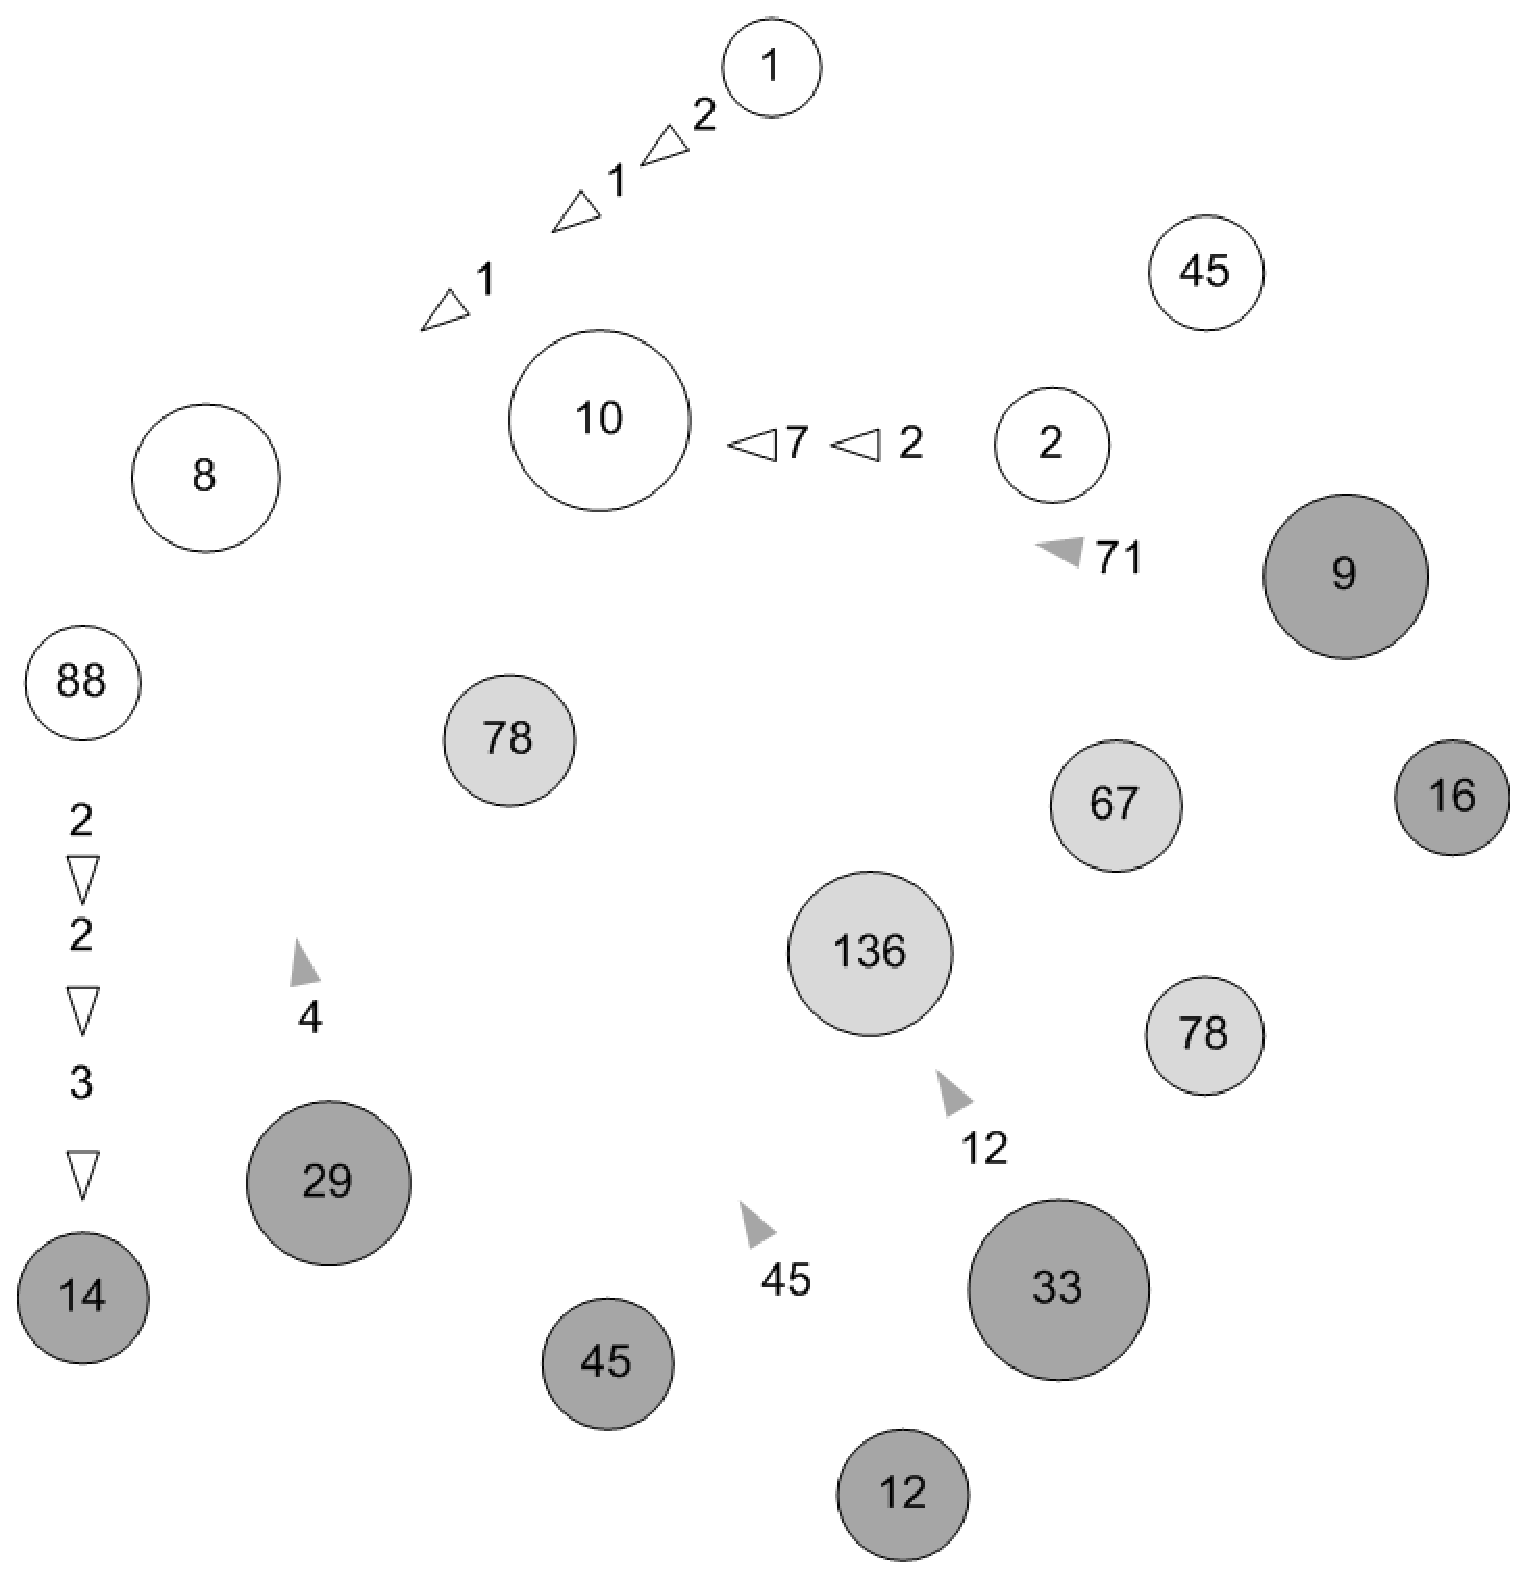
\epsfig{file=./imagenes/naves.eps,width=4cm}
\end{center}
\caption{Simulated screen shot of an early stage of a run in Planet Wars. White planets belong to the player (blue colour in the game), dark grey belong to the opponent (red in the game), and light grey planets belong to no player. The triangles are fleets, and the numbers (in planets and triangles) represent the ships. The planet size means growth rate of the amount of ships in it (the bigger, the higher).}
\label{figura:PlanetWars1}
\end{figure}

A Planet Wars match takes place on a map (see Figure \ref{figura:PlanetWars1}) that contains several planets (neutral, enemies or owned), each one of them with a number assigned to it that represents the quantity of ships that the planet is currently hosting. 

The aim of the game is to defeat all the ships in the opponent's planets. Although Planet Wars is a RTS game, this implementation has transformed it into a turn-based game, in which each player has a maximum number of turns to accomplish the objective. At the end of the match, the winner is the player that alives, or that owns more ships if more than one survives. 

% Maribel, las comas es que n ingl�s no se usan no? :-)

There are two strong constraints which determine the possible methods to apply to design
a bot: a simulated turn takes \textit{just one second}, and the bot is \textit{not allowed to store any kind of information} about its former actions, about the opponent's actions or about the state of the game (i.e., the game's map).

Therefore, the aim in this paper is to study the improvement of a bot according to the state of the map in each simulated turn (input), returning a set of actions to perform in order to fight the enemy, conquering its resources, and, ultimately, wining the game. In the original game, only two bots are faced but in this paper it is studied what happen when we simulate 4 on 4 battles, i.e., when 4 bots are fighting in the same map.


%%%%%%%%%%%%%%%%%%%%%%%%%%%%%%%%  CO-EVOLUTION  %%%%%%%%%%%%%%%%%%%%%%%%%%%%%%%%
%
\section{Cooperative and Competitive Evolution: Co-evolution}
\label{sec:co-genebot}

%Añadir referencias de Maribel:

There are two types of co-evolution, attend of the interaction between the individuals of the population: cooperative and competitive. In this paper, it's described an coevolutionary algorithm that has the two sides.

For one hand, are will % Maribel, are will??? eso qu� es " son ser�n" ???--- No uses el futuro, sino el presente o el pasado, no van a luchar, sino que ya han luchado. Lo he cambiado yo
simulated 4 on 4 battles were severals bots fight for the same goal: win the battle. That means that the bots compete against each other. Also, the individuals compete in the GA for perpetuate their species.

For other hand, the cooperative side come because the 4 on 4 battle is {$all\ versus\ all$}, so a single individual are allowed have assistance %cambio la expresi�n tener ayuda
from others for {$kill$} a temporally mutual rival. But beware, it is totally sure that at the end, only one is allowed. In addition, in the GA the individuals are sharing {$knowledge$}, because they are {$living$} (and fighting) together. If the population is improved, and the new individuals are {$born$} of these population, the new individuals will be better and better.

One of the major problems founded in the use of EAs for training bots for this behavior is %Maribel, lo pongo en presente, porque es un problema que existe ahora mismo, no que exist�a.
 the huge time needed for the evaluation, because we have to simulated full %Maribel, los adjetivos no llevan sssssssss, ya se la he quitado yo 
battles, in several maps, several times causes. In addition, when dealing with a noise and stochastic problem like this, it is forced to use re-evaluation between generations.

Theoretically, the use of a co-evolution allows %Maribel, falta la s
to reduce the number of simulations needed, because the population is evaluated in {$groups$}. That's, if there is % Maribel, es singular, la poblaci�n es una, quito el are 
a population of 100 individuals, in a classic GA it's needed make 100 evaluations, once for each individual, for each generation, times for the number of maps and the re-evaluation or others factors. In co-evolution case, for example, if it is used two bots of the population for the co-evolution we only need 50 evaluations. % ya has dicho al principio que es para el caso Co-GA, no hace falta repetir for the Co-GA. 
%Maribel, unas veces dices CGA y otras CoGA o Co-GA, hay que unificarlo
It is likely that simulations with four bots spent more time that a simulation with two bots, but the question is if the time taken for a {$4-simulations$} is less that the time taken for two {$2-simulation$}. In that case, the co-evolution decreases the time needed for the training.  % Maribel, aqu� falta una tablita de tiempos o algo que justifique lo que dices.

The use of two individuals or four individuals of the population in the experiments depends of the use (or not) of previous knowledge. 

\subsection{Previous Knowledge vs Auto-generated Knowledge}
\label{sec:knowledge}

It has an best training bot, %Maribel, it has an best? eso qu� es lo que es?
which has proved its worth in 1vs1 battles. The question is if can be used the previous knowledge for improving %Maribel, detr�s del for, va gerundio
 (faster) better bots in a similar problem. Or maybe, if it is best do not use previous knowledge and allow fight versus individuals of the population; that theoretically (as the bases of the GAs) will improve each generation. To answer this question, two types of experiments were designed.
%Maribel, he cambiado algunas cosas para que parezcan un poco m�s formales

\subsubsection{Co-evolution with previous Knowledge}
\label{sec:knowledge:previous}

In this case, battles between two individuals of the population versus two of the best bots (in 1vs1 contest) have been simulated. %Maribel, la frase anterior, no ten�a sujeto 
It is expected that the co-bots were able to learn the bases of the best bots, and improve for be better in 4 on 4 battles. It is desirable for this  co-evolution approach the algorithm rewards bots that at least won in a battle with the previous best bots. %Maribel, he cambiado la frase entera, hab�a mucho lio y alg�n fallo, espero no haber cambiado el sentido, as� que revisalo 

Regarding the execution time of this approach, we did not expect a great time reduction during the training of the bots, although it was desirable. 
%Maribel, cambio esta frase sin dar tanta vuelta. Talcking about the time needed for the execution, it's not expected an huge reduction of the time needed for the training of the bots, but it's desirable that happen. It's something that will be increased in the next co-evolution method.

\subsubsection{Co-evolution with Auto-generated Knowledge}

In this case, battles with four individuals of the population were tested. %will be simulated battles between four individuals of the population. 
For this approach the knowledge in included into the individual when it fights in previous battles, but the bots were improving for being better versus bots every generation improved (because the population is expected to be better in each generation). %Maribel, el will no tiene sentido, habla en pasado o en presente, no en futuro, es algo que ya est� hecho no que se va ha hacer.
%Maribel, de verdad que no entiendo lo que quieres decir en la �ltima frase, la frase no tiene muchos pies ni muchas cabezas, o yo no entiendo nada de nada.

Regarding the execution time of this approach,  we expect to reduce the needed time by $50\%$ respect to the previous approach, because it reduces the number of evaluations to the half.
%Maribel, reescribo esto: Talcking about the time, this method would reduce the time needed near to 50\% that the previous method, because it reduced the number of evaluations to the half.

\subsection{Fitness}

In previous works, a bot is evaluated always versus the same bot (an reference-bot). For fitness function, the bot is evaluated several times (in different maps). The fitness function is defined depending of the result of the battle (if the bot wins all its battles or loses in someone) and the numbers of turns needed for ending the game. For two bots, A and B the fitness is defined as the figure \ref{fig:fitness_turns_positions} shows \subref{fig:fitness_turns_positions:2}. 

%This fitness works well for 1vs1 battles, and the first fitness proposed is an natural evolution of this fitness applied to 4 on 4 bots battles.

\subsubsection{Fitness based in Position and turns}

This fitness is the natural evolution of the previous one, applied to 4 bots battles. Again, the evaluations are done with several maps. In this case, both the position ($1^{th}$, $2^{th}$,..) of the bot in the 4-battle and the number of used turns, are included into the study. % Maribel, la siguiente frase no se entiende, la voy a intentar reescribir, revisala por si cambio el sentido de algo.
%For a bot that wins all the battles (it's $1^{th}$ in all) it's call {$ferocity$} to the sum turns, in previous works was found that a bot that wins in less turns it's best that other that takes more turns in win too. 
We set the feature ferocity to each bot that wins all its battles. This ferocity  feature is included into the fitness as the sum of turns the bot need to win. This sum can be used to select the best bot when more than one wins all its battles because a bot that wins with less turns is better than other that wins all its battles but with more turns. 
In other cases, the sum of turns is called {$sturdy$}, and opposite to the {$ferocity$}, it is desirable a bot that take more turns in be defeated. In fig\ref{fig:fitness_turns_positions}(\subref{fig:fitness_turns_positions:2})there are an formal description of this fitness.

\begin{figure}[h]
\tiny
\begin{subfigure}[!]{0.5\textwidth}
\begin{algorithmic}
        \State{$A,B\in Population $}
        \If {A WINs always}
            \If{B LOSEs some battle}
                \State A is better than B
            \ElsIf{A take less turns than B}
                \State A is better than B
            \Else
                \State B is better than A
            \EndIf
        \Else
             \If{B WINs always}
                \State B is better than A
            \ElsIf{A take less turns than B}
                \State B is better than A
            \Else
                \State A is better than B
            \EndIf
        \EndIf
        \end{algorithmic}
        \label{fig:fitness_turns_positions:2}
\caption{Fitness used in battles of 2 bots}
\end{subfigure}
\begin{subfigure}[!]{0.5\textwidth}
    \begin{algorithmic}
        \State{$A,B\in Population $}
        \If {A average position $<$ B average position}
            \State A is better than B
        \ElsIf{A average position $>$ B average position}
            \State B is better than A
        \Else
            \If{A,B is always $1^{th}$}
                \If{A take less turns than B}
                    \State A is better than B
                \Else
                    \State B is better than A
                \EndIf
            \Else
                \If{A take less turns than B}
                    \State B is better than A
                \Else
                    \State A is better than B
                \EndIf
            \EndIf
        \EndIf
    \end{algorithmic}
    \label{fig:fitness_turns_positions:co}
\caption{Fitness used in battles of 4 bots}
\end{subfigure}
\label{fig:fitness_turns_positions}
\caption{Fitness based in turns and positions}
\end{figure}

In this fitness, we are only interesting in the final result: position and turn. We do not include into the analysis how the bot reach it. However, two variables are involved in the calculation of the fitness. Both variables make difficult the operation with severals evaluations, because the fitness is not possible to sum o average easyly. In the next fitness, it's used another metric to define the goodness of the bots. The percentage of the ships that in each turn belong to each player. 

For study the ships, we read from the simulation how many ships belong to each player in each turn, normalized at total ships in game for that turn (including neutrals ships in neutral planets). For each player, we have a different {$cloud$} like in Fig.\ref{figura:nubecita}. Below, see two alternatives to deal with this cloud of points for the fitness function: using slopes and areas.

\begin{figure}[h]
\begin{center}
  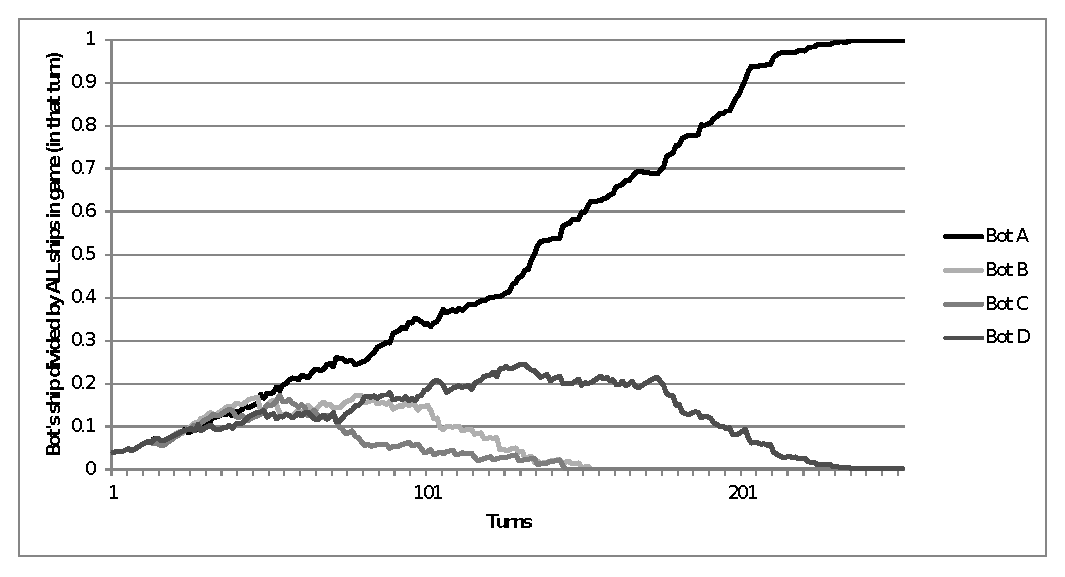
\epsfig{file=imagenes/nubecita.eps,width=4cm}
\end{center}
\caption{Representation of the number of ships of each bot in each turn} 
\label{figura:nubecita}
\end{figure}

\subsubsection{Fitness based in Slope}

For this fitness,  squares regression analysis for resume the cloud of points to a simple line, is calculated. A line is represented as {$y = \alpha \times x + \beta $}, where {$\alpha$} and {$\beta$} are calculated as show the Fig. \ref{equation:LeatsSqueares} according to least squares regression. For each bot in the simulation we calculate $\alpha$, ($slope$). This $slope$ is the fitness for each bot for that simulation.
%Maribel, he cambiado todos los it's que no s� por qu� los pones y he simplificado las frases

\begin{figure}[h]
\begin{subfigure}[H]{0.4\textwidth}
    \begin{equation}
        \alpha = \frac{\sum_{i=1}^{n}(X_{i} - \bar{X_{i}})(Y_{i} - \bar{Y_{i}})}{\sum_{i=1}^{n}(X_{i} - \bar{X_{i}})^{2}}
    \end{equation}
    \begin{equation}
        \beta = \bar{Y}-\alpha\bar{X}
    \end{equation}
    \caption{Leats squares regression}
    \label{equation:LeatsSqueares}
\end{subfigure}
\begin{subfigure}[H]{0.8\textwidth}
\begin{center}
  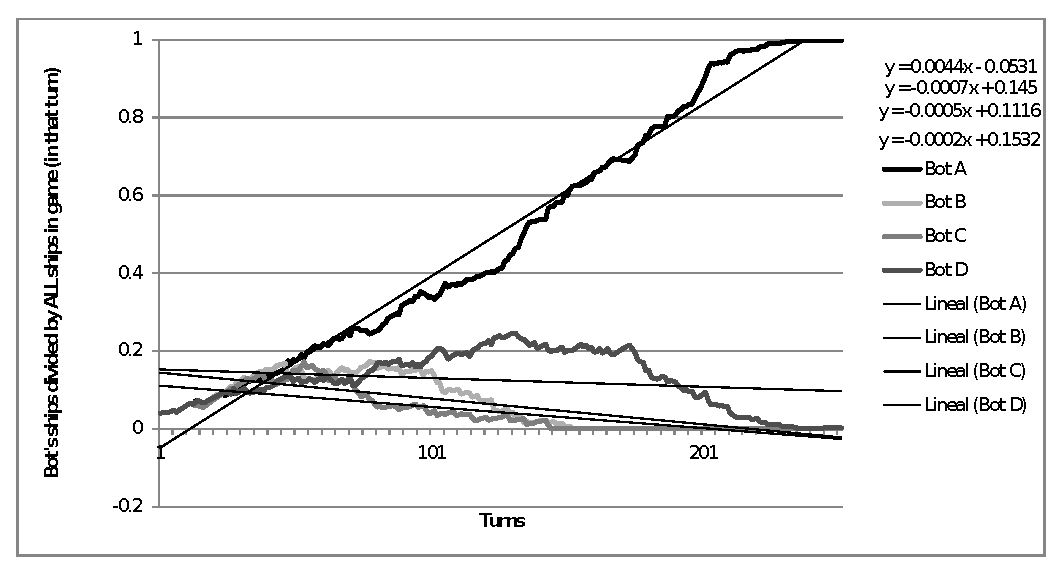
\epsfig{file=imagenes/nubecita_pendiente.eps,width=1\textwidth}
\end{center}
\caption{Representation of the number of ships of each bot in each turn} %Maribel, cambio if por of
\label{figura:nubecita}
\end{subfigure}
\end{figure}

A %Maribel, sin n
theoretical maximum an minimum values is fixed for this fitness. An optimum bot that wins in the first turn, has an slope of {$1$}, so this is the maximum value of our fitness. In the other hand, a bot that loses in the first turn,  has an slope of {$-1$}. In addition, if we calculate the $slope$, we know if the bot {$WINs$} ({$slope>0$}) or {$LOSEs$} {$slope<0$}. Finally, the bot with the closer to the maximum $slope$ should be the best is each turn or battle. %maribel he cambiado entera la frase anterior porque  no se entend�a nada

%Several evaluations in different maps was using, so it's need operate with fitness. In that case, only sum the slope of all the evaluations of the bot. Maribel, esto ya lo has dicho antes y adem�s l�a m�s la cosa as� que lo he eliminado. Adem�s expresiones como "was using" est�n mal, qu� quieres decir? fue usando? eso en ingl�s no se dice.

\subsection{Fitness bases in Area}
\label{sec:fitness}

For this case, the integral of the curve of the bot's live-line is used for calculate the area that is included into the fitness. This {$area$} is normalized to the number of turns, representing the average percentage of ships along the battle for each player. In the Fig\subref{equation:LeatsSqueares}
%Maribel, simplifico mucho la primera frase, porque ya todo el mundo deber�a saber que la integral es el �rea entre una curva y el eje x.

\begin{figure}[h]
\begin{subfigure}[H]{0.4\textwidth}
    \begin{equation}
        area=\frac{\int_{0}^{t}\%ships(x)dx}{t}
    \end{equation}
    \caption{Calculus of the area}
    \label{equation:LeatsSqueares}
\end{subfigure}
\begin{subfigure}[H]{0.8\textwidth}
\begin{center}
  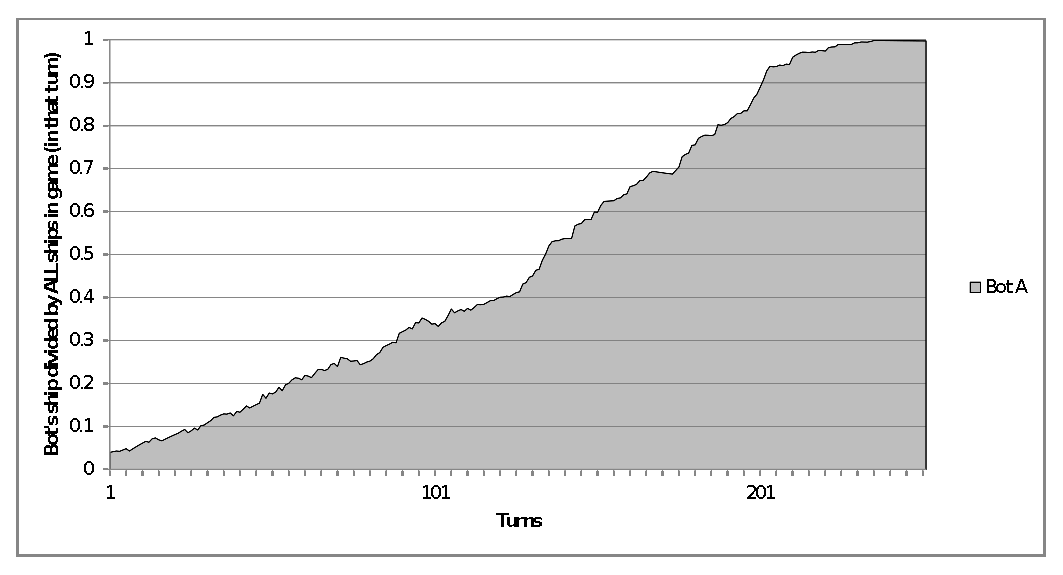
\epsfig{file=imagenes/nubecita_integral.eps,width=1\textwidth}
\end{center}
\caption{Example of area under the live-line curve.} 
\label{figura:nubecita}
\end{subfigure}
\end{figure}

As in the previous case, a theoretical maximum and minimum values are fixed for this fitness. if an optimal bot wins in the first turn, the area of each live-line is close to {$1$}, so this is the maximum value of the fitness. Furthermore, if a bot loses in the first turn, its live-line area is close to {$0$}. In this case, we do not extract addicional information related with which bot wins the battle, because the area of the live-line is not related with the winner of the battle. In this scope, we are losing some information.

% Maribel, he corregido-reescrito todo el p�rrafo anterior

%%%%%%%%%%%%%%%%%%%%%%%%%%%%%%%   EXPERIMENTS  %%%%%%%%%%%%%%%%%%%%%%%%%%%%%%%%
%
\section{Experiments and Results}
\label{sec:experiments}


%%%%%%%%%%%%%%%%%%%%%%%%%%%%%%  CONCLUSIONS  %%%%%%%%%%%%%%%%%%%%%%%%%%%%%%%
%
\section{Conclusions and Future Work}
\label{sec:conclusions}



%%%%%%%%%%%%%%%%%%%%%%%%%%%%%%   ACKNOWLEDGEMENTS %%%%%%%%%%%%%%%%%%%%%%%%%%%%%%

\section*{Acknowledgements}

This paper has been funded in part by projects P08-TIC-03903 (Andalusian Regional Government), TIN2011-28627-C04-02 (Spanish Ministry of Science and Innovation), and project 83 (CANUBE) awarded by the CEI-BioTIC UGR.

\bibliographystyle{splncs}
\bibliography{genebot}


\end{document}
